\chapter{TiO Line Measurements} % Main appendix title
\protect\label{chapter:tioline}
\lhead{Appendix \ref{chapter:tioline}. \emph{Tio Line}}

A prominent absorption line consistent across the spectra was identified to be a TiO transition at 6572.468{\AA} to
6573.288{\AA}, highlighted as the dark green shading in the right panel of Fig. \ref{fig:harps2}. This is enlarged
in Fig. \ref{fig:tispec}. The equivalent widths of this line from the {\harps} data and also a version of the peak
ratios in the same manner as for Table \ref{table:ewtabfirst}. Results are shown in Table \ref{table:titable}.
\examrevision{Attempts were made to derive periodograms in the same manner as for {\ha} but no clear-cut results were obtained.}

\begin{figure}[!htbp]
\begin{center}
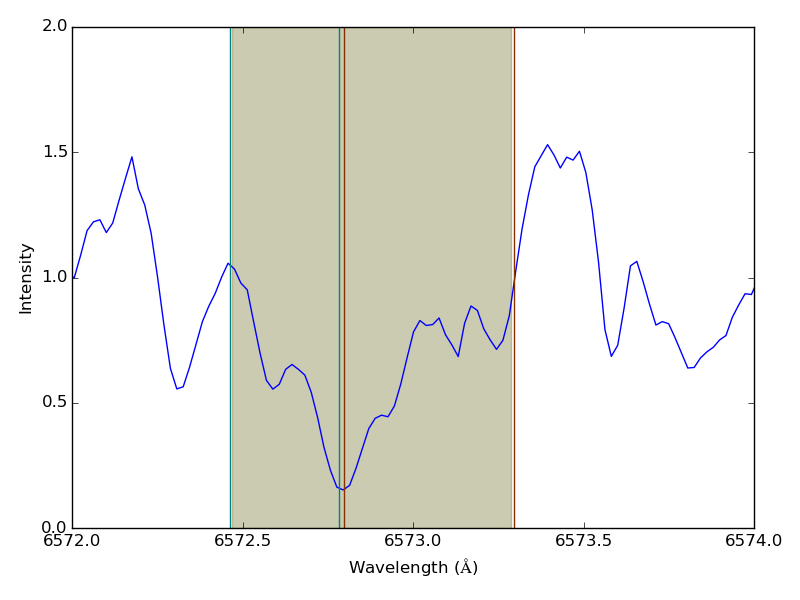
\includegraphics[scale=0.25]{Figures/tispec.png} \\
\end{center}   
\caption{This shows the section of the first spectrum in the {\harps} data (at 27 May 2004 UTC 02:10:14) used for
  calculating Equivalent Widths and also Peak Ratios from the TiO absorption line from 6572.468{\AA} to
  6573.288{\AA}. The blue vertical lines at 6572.463{\AA} and 6572.784{\AA} and the red lines at 6572.797{\AA} and
  6573.295{\AA} delineate the regions used for calculation of a version of the Peak Ratios.}
\protect\label{fig:tispec}
\end{figure}

\begin{table}[!htbp]
\centering
\scalebox{0.75}{
\begin{tabular}{|l|l|r|c|c|c|}
\hline
From & To & No. & EW  & Index & PR \\\hline
27/05/2004 & 21/07/2004 & 6 & 0.309 $ \pm $ 0.019 & 0.032 $ \pm $ 0.002 & 1.039 $ \pm $ 0.027 \\
25/07/2005 & 22/03/2006 & 5 & 0.314 $ \pm $ 0.004 & 0.032 & 1.017 $ \pm $ 0.012 \\
14/03/2007 & 19/07/2007 & 5 & 0.310 $ \pm $ 0.006 & 0.032 $ \pm $ 0.001 & 1.030 $ \pm $ 0.036 \\
29/06/2008 & 06/04/2010 & 25 & 0.315 $ \pm $ 0.007 & 0.031 $ \pm $ 0.001 & 1.020 $ \pm $ 0.035 \\
19/02/2011 & 03/06/2011 & 12 & 0.312 $ \pm $ 0.008 & 0.032 $ \pm $ 0.001 & 1.036 $ \pm $ 0.024 \\
18/01/2013 & 10/01/2014 & 207 & 0.310 $ \pm $ 0.006 & 0.032 $ \pm $ 0.001 & 1.047 $ \pm $ 0.027 \\
19/01/2016 & 30/03/2016 & 56 & 0.319 $ \pm $ 0.015 & 0.031 $ \pm $ 0.001 & 1.005 $ \pm $ 0.028 \\\hline
\multicolumn{2}{|c|}{ALL} & 316 & 0.312 $ \pm $ 0.010 & 0.032 $ \pm $ 0.001 & 1.036 $ \pm $ 0.033 \\\hline
\end{tabular}}
\caption{Results for calculation of median and standard deviation of the equivalent widths of the TiO transition at 6572.468{\AA} to
6573.288{\AA} from \harps. The observations are separated where they are 300 or more days apart.}
\protect\label{table:titable}
\end{table}

As Table \ref{table:titable} shows, an ``index'' was also considered along the same lines as the {\ha} Index, but the
size and variations (0.032 $\pm$ 0.001) were far too small to be useful.
